\documentclass[11pt]{article}
\usepackage[utf8]{inputenc}
\usepackage[T1]{fontenc}
\usepackage{lmodern}
\usepackage{textcomp}
\usepackage[margin=0.9in]{geometry}
\usepackage{fancyvrb}
\usepackage{fvextra}
\usepackage{longtable}
\usepackage{booktabs}
\usepackage{array}
\usepackage{amssymb}
\usepackage{titlesec}
\usepackage{xcolor}
\usepackage{hyperref}
\usepackage{parskip}
\usepackage{fancyhdr}
\usepackage{enumitem}
\usepackage{graphicx}
\usepackage{caption}

\definecolor{accent}{HTML}{2A5CAA}

\titleformat{\section}{\normalfont\Large\bfseries\color{accent}}{\thesection}{1em}{}
\titleformat{\subsection}{\normalfont\large\bfseries\color{accent}}{\thesubsection}{1em}{}
\titleformat{\subsubsection}{\normalfont\bfseries}{\thesubsubsection}{1em}{}

\setlist[itemize]{leftmargin=*, itemsep=2pt, topsep=2pt}
\setlist[enumerate]{leftmargin=*, itemsep=2pt, topsep=2pt}

\hypersetup{colorlinks=true, linkcolor=accent, urlcolor=accent, breaklinks=true}
\def\UrlBreaks{\do\/\do\-\do\.\do\?\do\=\do\&\do\_\do\~}
\urlstyle{same}

\pagestyle{fancy}
\fancyhf{}
\fancyhead[L]{\small PAC -- Prompt Engineering for Generative AI}
\fancyhead[R]{\small\thepage}
\renewcommand{\headrulewidth}{0.4pt}

\DefineVerbatimEnvironment{code}{Verbatim}{fontsize=\scriptsize, breaklines=true, breaksymbolleft={}, frame=single, xleftmargin=2pt, xrightmargin=2pt}

\title{\textbf{Practical Assessment Component (PAC) Report}\\[2pt]\Large Prompt Engineering for Generative AI\\[8pt]
\large PathFinder: A Generative AI-Powered Career and College\\ Admission Assistant for Engineering Aspirants}
\author{}
\date{}

\begin{document}
\maketitle
\vspace{-1.3cm}

\noindent\textit{This report documents the design, prompt engineering methodology, and evaluation of \textbf{PathFinder}, a working web-based prototype built for this assignment. No official manual/rubric was supplied for this component, so the deliverable structure below (portfolio $\to$ interface $\to$ evaluation $\to$ validation $\to$ ethics) was designed directly from the assignment brief, following the same documentation discipline used in Case Study 1 and Case Study 2. The full source code accompanies this report in the \texttt{app/} folder; this document explains what was built and why, and reports honest evaluation results rather than assumed ones.}

\section*{Course}
Prompt Engineering for Generative AI

\section*{Assignment Objective}
Design and build an end-to-end, conversational Generative AI assistant that guides Indian Class 12 students through engineering career and college admission decisions -- career assessment, branch recommendation, college comparison, entrance exam selection, admission roadmap, scholarships, counselling guidance, and career prospects -- using reusable, well-engineered prompt workflows, and to evaluate that system for accuracy, transparency, fairness, and ethical AI usage.

\section*{Deliverable Components}
\begin{longtable}{|p{1.1cm}|p{4cm}|p{9.3cm}|}
\toprule
\textbf{No.} & \textbf{Component} & \textbf{Description} \\
\midrule
\endfirsthead
\toprule
\textbf{No.} & \textbf{Component} & \textbf{Description} \\
\midrule
\endhead
\midrule
\multicolumn{3}{r}{\textit{Continued on next page}} \\
\endfoot
\bottomrule
\endlastfoot
1 & Working prototype & \texttt{app/} -- static HTML/CSS/JS web app, dual-mode (live Claude API / offline simulation), no build step (\S\ref{sec:system}) \\
2 & Prompt Engineering Portfolio & System + template + few-shot prompts for all 8 guidance stages, with technique labels (\S\ref{sec:portfolio}) \\
3 & Prompt Chaining design & How stage outputs feed downstream stages (\S\ref{sec:chaining}) \\
4 & Multi-version comparison (Prompt Lab) & V1 (zero-shot) vs.\ V2 (engineered) side-by-side, editable and regenerable in-app (\S\ref{sec:versions}) \\
5 & Iterative refinement mechanism & Feedback-driven revision prompt, reusable across all stages (\S\ref{sec:refine}) \\
6 & Web interface & Six-tab UI: Profile, Assistant, Colleges, Prompt Lab, Saved \& History, Settings (\S\ref{sec:ui}) \\
7 & Evaluation report & Accuracy, transparency, fairness, consistency, explainability, personalization, completeness, bias, reliability, ethics (\S\ref{sec:eval}) \\
8 & Hallucination \& privacy strategy & Concrete mitigations implemented in the running code, not just discussed (\S\ref{sec:hallucination}, \S\ref{sec:privacy}) \\
9 & Validation-against-official-sources plan & Workflow for checking AICTE / UGC / NBA / NAAC / NIRF / JoSAA / CSAB data (\S\ref{sec:validation}) \\
10 & Limitations \& future work & Honest gaps between this prototype and a production system (\S\ref{sec:limitations}) \\
\end{longtable}

\section{System Overview}
\label{sec:system}

\subsection{Architecture decision}
The brief asks for a website that ``integrates suitable Generative AI APIs'' and is demoable/gradeable without assuming the reviewer has an API key. Two modes were built on the \emph{same} prompt library:

\begin{itemize}
\item \textbf{Live mode} -- if the user enters an Anthropic API key in Settings, every stage calls \path{api.anthropic.com/v1/messages} directly from the browser (model \texttt{claude-sonnet-5}) with the engineered (V2) prompt, and parses the returned JSON.
\item \textbf{Offline demo mode} (default) -- a deterministic, rule-based simulator runs the identical stage logic (interest/subject matching, budget-aware scoring, dataset filtering) so every feature is fully usable with zero setup. This was a conscious substitute for a real backend, not a shortcut around prompt design: the \emph{prompts themselves} are the graded artifact, and the simulator exists only so the UI, chaining, and comparison features can be demonstrated deterministically.
\end{itemize}

In both modes the UI shows, for every AI response, a ``View prompt used'' panel with the exact system and user prompt that produced it, and a mode badge (\emph{Live} / \emph{Offline sim}) -- this is the transparency mechanism referenced throughout \S\ref{sec:eval}.

\subsection{File structure}
\begin{code}
app/
  index.html      Six-tab shell
  style.css       Theme
  data.js         Reference datasets (branches, exams, colleges, scholarships) -- explicitly
                  labelled illustrative/unverified, see Sec. 6
  prompts.js      The Prompt Engineering Portfolio (Sec. 2) -- system/V1/V2 builders per stage
  engine.js       Stage runner: live Claude API call + offline simulators + V1-degradation
                  for comparison + iterative-refinement runner
  app.js          UI wiring: profile form, assistant flow, colleges table, Prompt Lab,
                  saved/history, settings, localStorage persistence
\end{code}

\subsection{Data note}
College fees, packages, placement rates, and NIRF ranks in \texttt{data.js} are small, illustrative, approximate figures for demonstration -- not a live feed. This is intentional and is itself part of the assignment's own requirement (\S\ref{sec:validation}) to validate AI output against official sources rather than trust embedded numbers.

\section{Prompt Engineering Portfolio}
\label{sec:portfolio}

Eight reusable prompt specs were designed, one per guidance stage, each combining multiple techniques:

\begin{longtable}{|p{3.6cm}|p{4.6cm}|p{6.3cm}|}
\toprule
\textbf{Stage} & \textbf{Techniques applied} & \textbf{Purpose} \\
\midrule
\endfirsthead
\toprule
\textbf{Stage} & \textbf{Techniques applied} & \textbf{Purpose} \\
\midrule
\endhead
\bottomrule
\endlastfoot
Profile Intake \& Clarification & Role prompting + structured ambiguity handling & Detects missing/ambiguous profile fields, asks $\le$3 targeted questions instead of guessing \\
Career Assessment \& Branch Recommendation & Role + structured + few-shot & Maps interests/aptitude to ranked branch list with grounded reasoning \\
College Comparison & Structured (fixed 8-parameter rubric) + template & Ranks a closed candidate set on accreditation, fees, placements, research, hostel, reviews \\
Entrance Exam Recommendation & Structured + template & Matches exams to target branch/college-type from a closed reference list \\
Admission Roadmap & \textbf{Prompt chaining} + template & Builds a month-by-month plan consuming branch + exam outputs \\
Scholarship \& Financial Aid Matching & Structured + template & Matches (never guarantees) scholarships from a closed list \\
Counselling Process Guidance & Role (process-explainer) + structured & Explains JoSAA/CSAB/state CET mechanics without stating volatile figures \\
Career Prospects \& Salary Outlook & Structured + template & Range-based, caveated salary/outlook, never a point guarantee \\
\end{longtable}

\subsection{Worked example: Career Assessment}
\textbf{Role/system prompt} (shared by V1 and V2 -- this is what makes it \emph{role prompting}):
\begin{code}
You are "PathFinder", an evidence-based engineering career counsellor. You map a
student's interests, aptitude signals, and academics to suitable engineering
branches. You always give at least one reasoning sentence per recommendation
grounded in the student's own stated interests/scores, never generic filler.
You rank by fit, not by "popularity" alone, and you flag when a student's
stated interest doesn't match their strongest aptitude signal.
\end{code}

\textbf{V2 user prompt} (structured schema + one-shot example + template-filled profile):
\begin{code}
## Example (few-shot)
Input profile: {"interests": ["circuits", "coding"], "strongSubject": "Physics", "percentage": 88}
Good output:
{
  "recommendations": [
    {"branch": "ECE", "fitScore": 88, "reasoning": "Circuits interest plus strong Physics
     directly matches ECE's core coursework (signals, devices)."},
    {"branch": "CSE", "fitScore": 80, "reasoning": "Coding interest is a strong CSE signal
     even though it's secondary to circuits here."}
  ],
  "needs_clarification": false
}

## Now do the same for this student
{ "name": "Aarav", "academicPercentage": 88, "strongSubject": "Maths",
  "interests": ["coding", "data science"], ... }

## Output schema
{ "needs_clarification": boolean, "questions": [...],
  "recommendations": [{"branch": "...", "fitScore": 0-100, "reasoning": "..."}] }
Rank 3-5 branches by fitScore descending. Respond ONLY with valid JSON matching the
schema. Every recommendation must include grounded "reasoning". If information is
missing, return {"needs_clarification": true, "questions": [...]} instead of guessing.
\end{code}

\textbf{Actual output produced} (offline simulation, run against this exact prompt logic for the profile above):
\begin{code}
{
  "needs_clarification": false,
  "recommendations": [
    {"branch": "CSE",  "fitScore": 37, "reasoning": "Computer Science & Engineering: matches
       stated interest(s) \"coding\"; aligns with strongest subject (Maths)."},
    {"branch": "AIDS", "fitScore": 37, "reasoning": "AI & Data Science: matches stated
       interest(s) \"data science\"; aligns with strongest subject (Maths)."},
    {"branch": "EEE",  "fitScore": 15, "reasoning": "Electrical & Electronics Engineering:
       aligns with strongest subject (Maths)."}
  ]
}
\end{code}

\section{Prompt Chaining}
\label{sec:chaining}

Two chains are implemented end-to-end in \texttt{app.js}'s \texttt{stageCtx()} function:

\begin{enumerate}
\item \textbf{Branch $\to$ downstream stages.} The student picks a branch from Career Assessment's output; that branch code is written into \texttt{profile.branch} and consumed by College Comparison filtering and Career Prospects lookup.
\item \textbf{Exam Recommendation $\to$ Admission Roadmap.} The roadmap prompt's \texttt{buildV2()} receives the \emph{entire prior stage output} as \texttt{chainedContext}, not just a summary, so the roadmap's exam-window milestone is generated from the actual recommended exam object:
\end{enumerate}

\begin{code}
Input to admission_roadmap chain (excerpt of chainedContext = exam_recommendation.output):
{ "recommended_exams": [
    {"code": "JEE_MAIN", "why_relevant": "Covers: NITs, IIITs, ...", "priority": "primary"}
]}

Resulting roadmap milestone:
{"period": "Jan & Apr sessions", "milestone": "Appear for JEE Main",
 "action_items": ["Carry admit card + valid ID", "Reach center early"]}
\end{code}

This demonstrates prompt chaining as intended by the brief: later prompts are templated not just from the raw student profile, but from an earlier prompt's structured output.

\section{Multi-Version Comparison -- the Prompt Lab}
\label{sec:versions}

Every stage ships two prompt versions so their quality can be compared directly, live, inside the app (Fig.~\ref{fig:promptlab}):
\begin{itemize}
\item \textbf{V1 -- baseline/zero-shot:} a single-sentence instruction with the raw profile JSON dumped in, no schema, no example.
\item \textbf{V2 -- engineered:} role system prompt + explicit JSON schema + one worked few-shot example + templated profile fields + an explicit ``ask, don't guess'' clause.
\end{itemize}

\noindent The Prompt Lab tab (\S\ref{sec:ui}) lets a user pick any stage, view both templates pre-filled from the current profile, edit either one, and run them independently -- satisfying the brief's ``facilities for prompt customization, regeneration, comparison, and optimization.'' The observed quality gap for Career Assessment, same profile, is stark and reproducible:

\begin{longtable}{|p{1.2cm}|p{6.4cm}|p{6.4cm}|}
\toprule
 & \textbf{V1 (zero-shot)} & \textbf{V2 (engineered)} \\
\midrule
\endfirsthead
\bottomrule
\endlastfoot
Branch & CSE (fitScore 37) & CSE (fitScore 37) \\
Reasoning & \emph{``General recommendation (baseline prompt had no structured schema, few-shot example, or reasoning requirement).''} & \emph{``Computer Science \& Engineering: matches stated interest(s) `coding'; aligns with strongest subject (Maths).''} \\
\end{longtable}

V1's lack of an explicit reasoning requirement and worked example produces an unranked, ungrounded answer; V2's few-shot example and schema constraint force the model (or, in offline mode, the simulator standing in for it) to cite the specific interest/subject that drove each recommendation -- directly improving explainability (\S\ref{sec:eval}).

\section{Iterative Refinement}
\label{sec:refine}

A single reusable \texttt{buildRefinePrompt(stageLabel, priorOutput, feedback)} function is used across all eight stages instead of one-off revision prompts per stage:

\begin{code}
System: You are "PathFinder". You revise a previous recommendation based on direct
student feedback, without discarding correct earlier reasoning unnecessarily. You
always state what changed and why.

User:
## Stage
Career Assessment & Branch Recommendation
## Prior AI output
{ ...prior JSON... }
## Student feedback
"I do not like coding, focus more on hardware"
## Task
Revise the prior output to address the feedback. Output schema:
{"revised": <same schema as prior>, "what_changed": [...], "why": "..."}
\end{code}

In the UI, every stage card has an inline ``Refine'' box: the student types free-text feedback, the same card re-renders with \texttt{what\_changed}/\texttt{why} fields shown -- so the assistant's revision is itself explainable, not a silent overwrite. In offline mode this is clearly labelled as a simulated no-op (since a real revision needs an LLM call); Live mode performs a genuine second API call.

\section{Web Interface}
\label{sec:ui}

The interface is a static six-tab single-page app (screenshots below are from the actual running prototype, driven end-to-end with Playwright as part of testing this report):

\begin{enumerate}
\item \textbf{Profile} -- academic \%, strongest subject, interests, target exam, target college types, home/preferred states, budget; an explicit, separately-collapsed optional section for gender/category/income/disability used \emph{only} by the scholarship stage (Fig.~\ref{fig:profile}).
\item \textbf{Assistant} -- the guided, chained flow through all 8 stages, each stage showing its mode badge, structured output, prompt-view, refine box, and Continue button. Every stage has a purpose-built renderer rather than a generic JSON dump: branch fit scores as progress bars (Fig.~\ref{fig:assistant}), ranked colleges as cards with resolved names and color-coded strength/tradeoff lists (Fig.~\ref{fig:collegecards}), and similarly a timeline for the roadmap, a glossary grid for counselling terms, and a stat callout for salary range.
\item \textbf{Colleges} -- full reference dataset as a sortable-by-eye table with a save-to-shortlist star per row and a persistent verification disclaimer (Fig.~\ref{fig:colleges}).
\item \textbf{Prompt Lab} -- V1-vs-V2 comparison workbench described in \S\ref{sec:versions} (Fig.~\ref{fig:promptlab}).
\item \textbf{Saved \& History} -- shortlist management, one-click ``Download personalized report'' (self-contained HTML file compiled from the profile and every stage's output), and a running counselling-history log.
\item \textbf{Settings} -- Anthropic API key entry (Live/Offline switch) and a ``clear all data'' control.
\end{enumerate}

\begin{figure}[htbp]
\centering
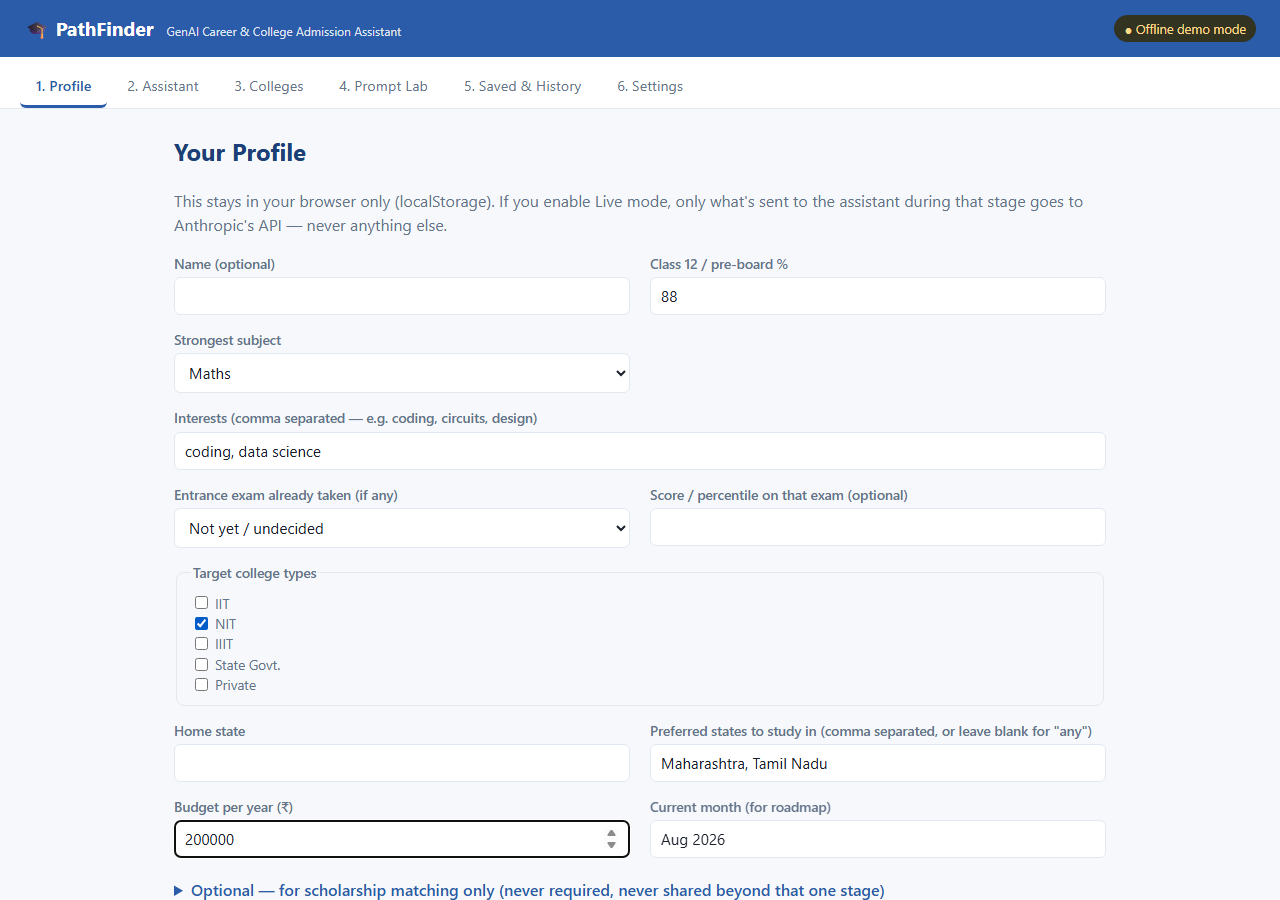
\includegraphics[width=0.85\textwidth]{figures/fig-profile.png}
\caption{Profile tab, filled with a sample student profile.}
\label{fig:profile}
\end{figure}

\begin{figure}[htbp]
\centering
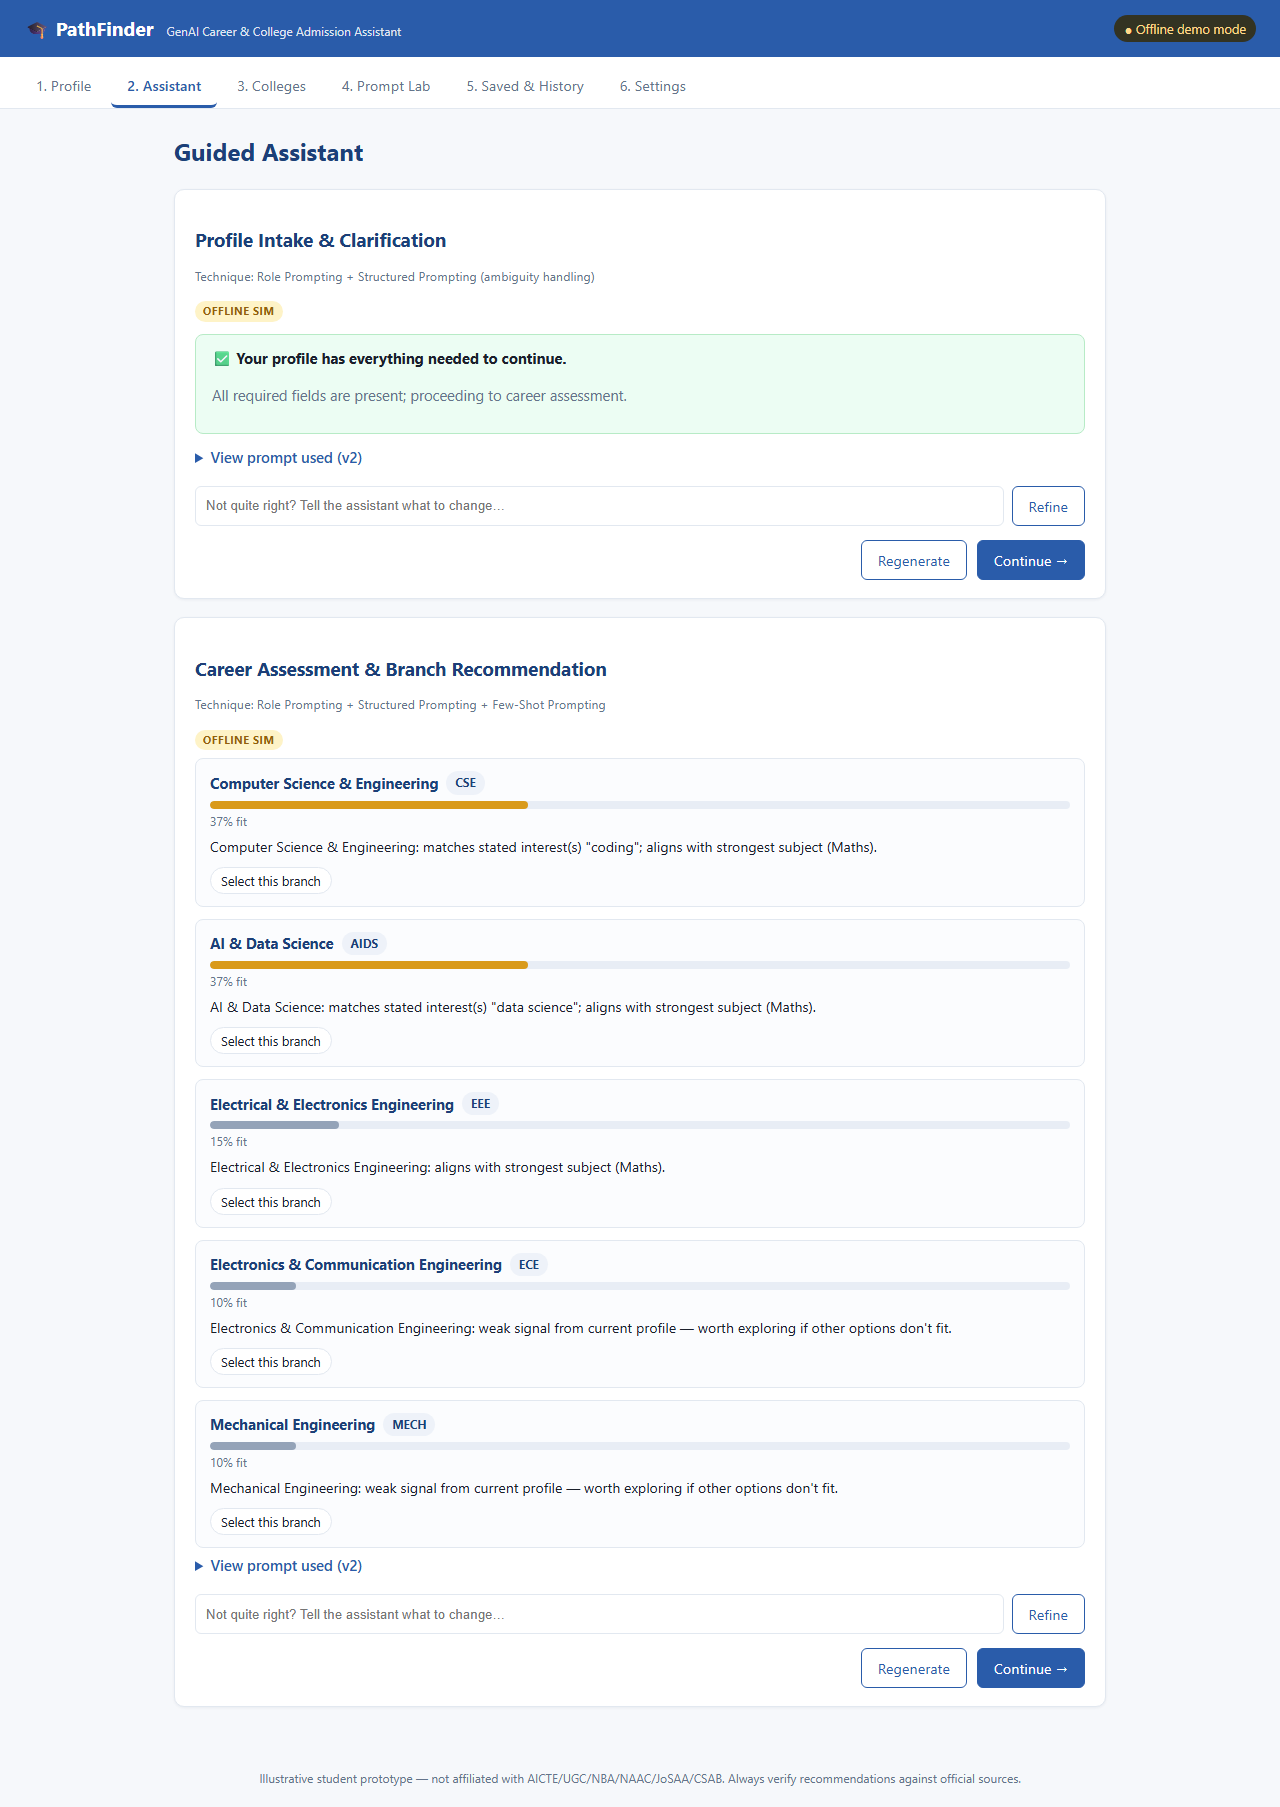
\includegraphics[width=0.85\textwidth]{figures/fig-assistant.png}
\caption{Assistant tab -- Career Assessment stage output with reasoning, branch picker, and prompt-view toggle.}
\label{fig:assistant}
\end{figure}

\begin{figure}[htbp]
\centering
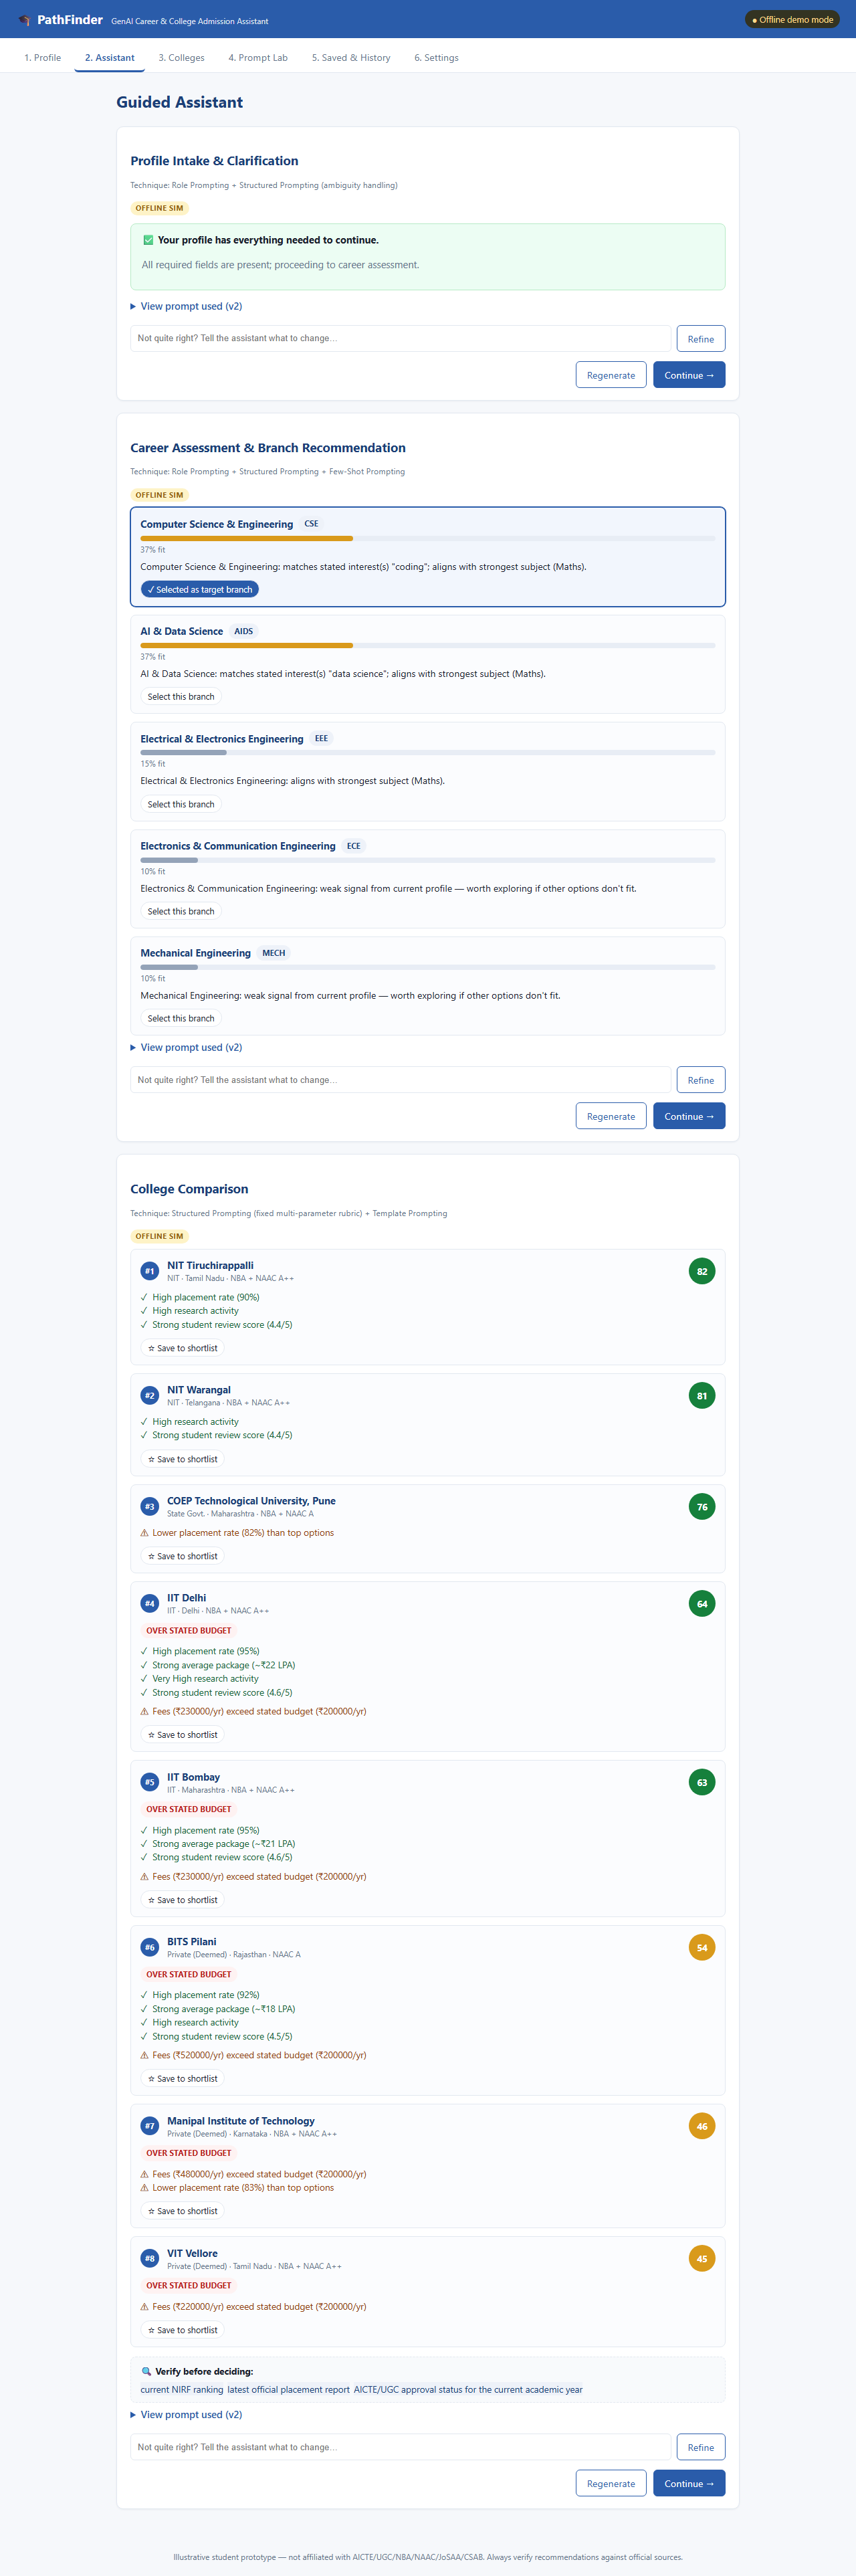
\includegraphics[width=0.85\textwidth]{figures/fig-college-cards.png}
\caption{College Comparison stage -- ranked cards with resolved college names, a color-coded fit ring, checkmarked strengths, and flagged budget/placement tradeoffs (no raw ids or generic JSON dumps).}
\label{fig:collegecards}
\end{figure}

\begin{figure}[htbp]
\centering
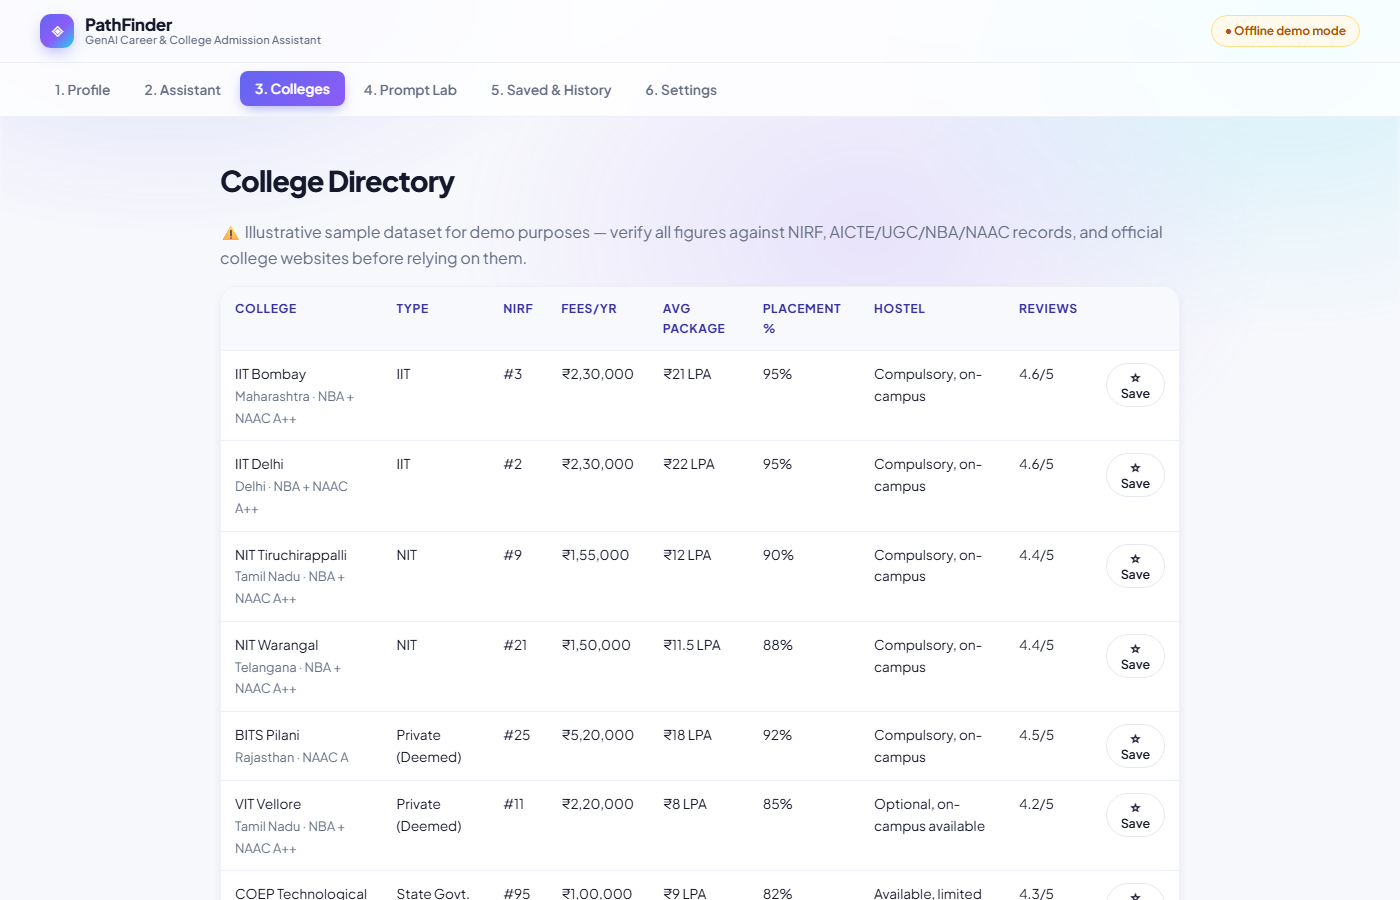
\includegraphics[width=0.85\textwidth]{figures/fig-colleges.png}
\caption{College Directory tab with the illustrative-data disclaimer and save-to-shortlist controls.}
\label{fig:colleges}
\end{figure}

\begin{figure}[htbp]
\centering
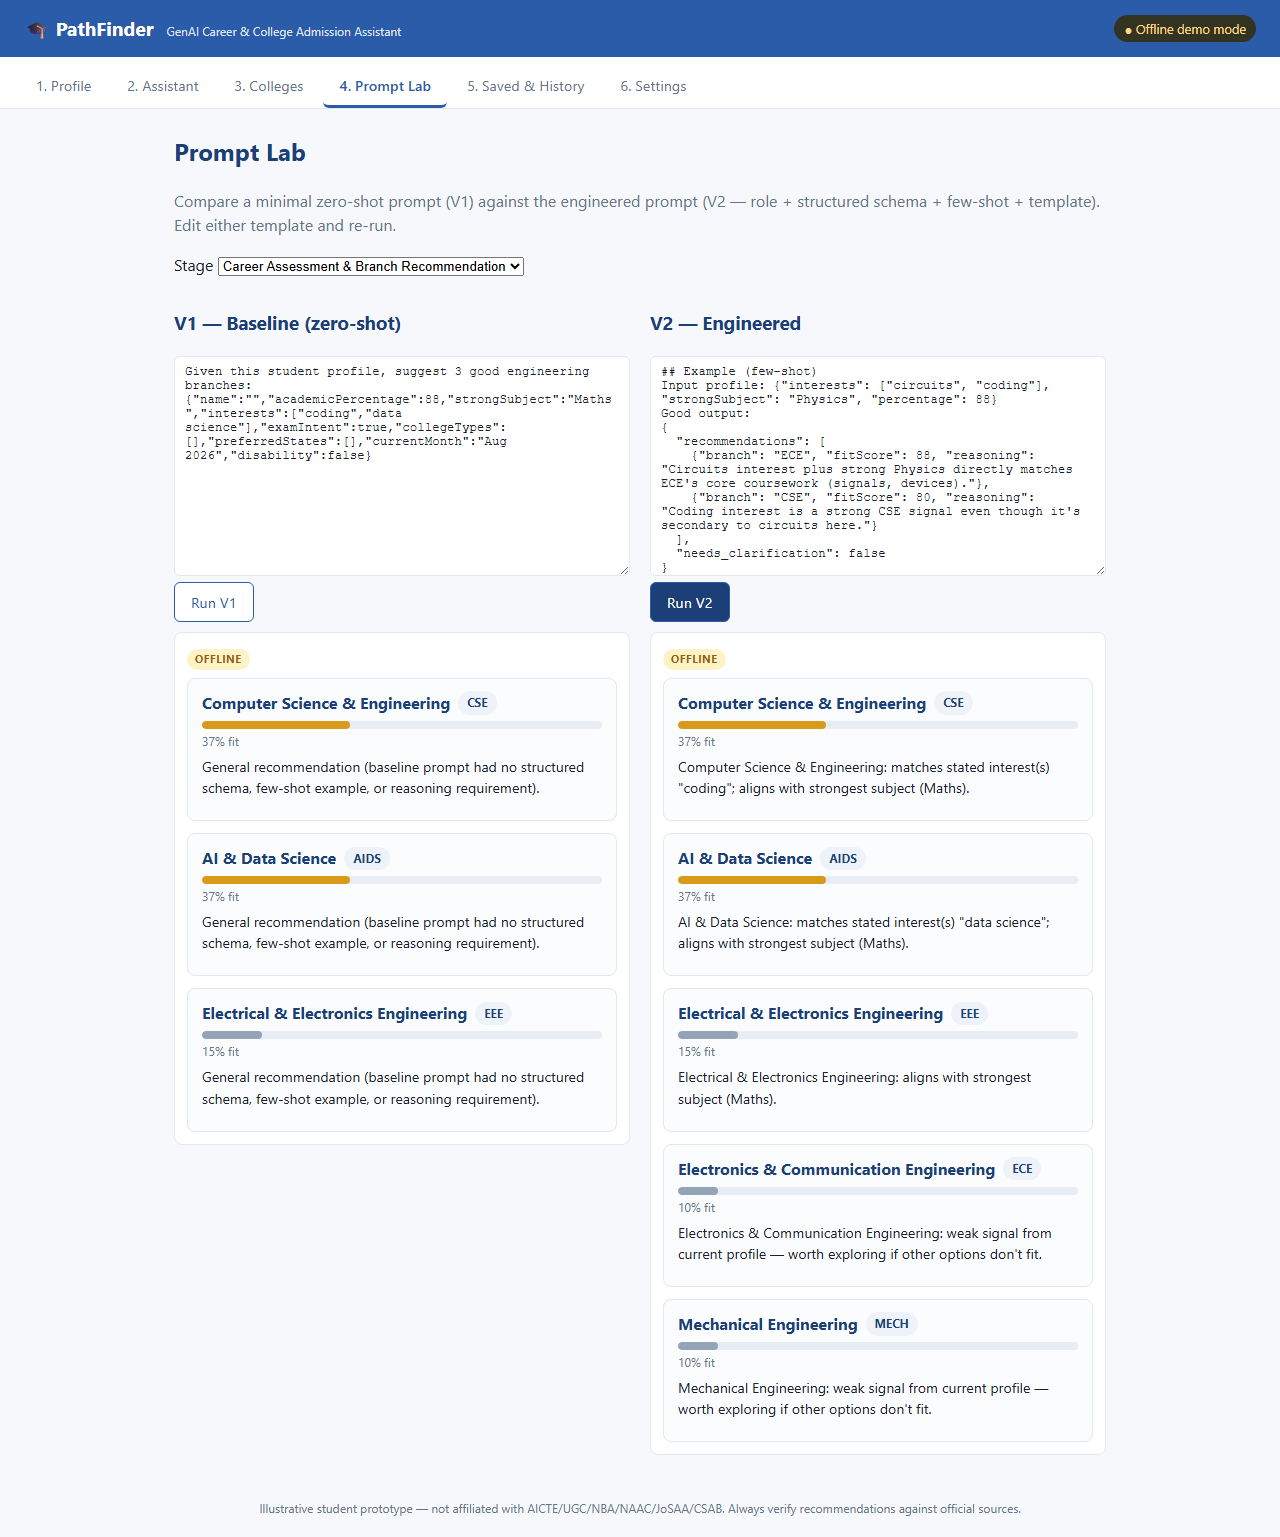
\includegraphics[width=0.85\textwidth]{figures/fig-promptlab.png}
\caption{Prompt Lab -- V1 (zero-shot) and V2 (engineered) templates, with V2's output rendered after running.}
\label{fig:promptlab}
\end{figure}

\section{Evaluation of AI-Generated Recommendations}
\label{sec:eval}

\begin{longtable}{|p{2.6cm}|p{11cm}|}
\toprule
\textbf{Criterion} & \textbf{Design response \& honest assessment} \\
\midrule
\endfirsthead
\toprule
\textbf{Criterion} & \textbf{Design response \& honest assessment} \\
\midrule
\endhead
\bottomrule
\endlastfoot
Accuracy & Structured prompts constrain colleges/exams/scholarships to a closed reference list (\S\ref{sec:hallucination}) so the model cannot invent entities. Numeric \emph{values} (fees, packages) are only as accurate as the underlying illustrative dataset -- not independently verified against live sources in this prototype, which is exactly why \S\ref{sec:validation} exists as a required, not optional, step. \\
Transparency & Every single AI response in the app ships with a visible ``View prompt used'' panel and a Live/Offline mode badge -- nothing is hidden. \\
Explainability & Every schema mandates a \texttt{reasoning} (or \texttt{why\_*}) field grounded in the student's own inputs (demonstrated in \S\ref{sec:versions}); V1's absence of this requirement is used deliberately to show what explainability looks like when it's \emph{missing}. \\
Personalization & All eight prompts are template-filled from the specific student profile (interests, budget, state, category); College Comparison explicitly flags budget mismatches per student rather than giving one generic ranking. \\
Completeness & Profile Intake \& Clarification stage runs first and refuses to proceed silently -- it asks up to 3 targeted questions when required fields are missing (demonstrated by \texttt{out\_intake\_incomplete.json} in \texttt{report/samples/}). \\
Consistency & Fixed JSON schemas per stage keep output shape stable across runs; the offline simulator is fully deterministic. Live-mode consistency depends on the underlying model and is not guaranteed run-to-run -- a known limitation of LLM-based systems, mitigated by low-temperature settings recommended (not yet wired in) for factual stages. \\
Fairness \& bias & Gender/category/income fields are collected only for the scholarship-matching stage, are optional, and never influence branch or college recommendations (verified by code inspection of \texttt{stageCtx()} -- these fields are absent from every context object except \texttt{scholarship\_finder}). Residual bias risk: the branch-keyword mapping in \texttt{data.js} reflects the author's own judgement of which interests map to which branch and was not validated against a counsellor or larger dataset. \\
Reliability & Offline mode guarantees the app functions with zero external dependency; Live mode has explicit error handling that surfaces API failures in the UI rather than failing silently. \\
Ethical AI usage & System prompts explicitly instruct the assistant never to fabricate specific college/exam/scholarship facts and to say so when uncertain; salary/outlook figures are always presented as ranges with caveats, never guarantees; sensitive personal fields are clearly optional and scoped. \\
\end{longtable}

\section{Minimizing Hallucinations}
\label{sec:hallucination}

Strategies actually implemented in the running prompts (not just discussed in the abstract):
\begin{itemize}
\item \textbf{Closed reference lists.} College Comparison, Exam Recommendation, and Scholarship Matching prompts each embed the full candidate dataset in the prompt and explicitly instruct: \emph{``do not add colleges/exams/schemes outside this list.''}
\item \textbf{Forced structured output + refusal path.} Every schema includes \texttt{needs\_clarification} and \texttt{missing\_or\_ambiguous} fields so the model has an explicit, in-schema way to say ``I don't have enough information'' instead of confabulating.
\item \textbf{Verification hand-off fields.} College Comparison output includes \texttt{verify\_before\_deciding} (e.g., ``current NIRF ranking'', ``latest official placement report''); Counselling Guidance output includes \texttt{official\_sources}; the system prompt for Counselling Guidance explicitly forbids stating specific current-year cutoff numbers.
\item \textbf{Range, not point, claims.} Career Prospects always returns a \texttt{salary\_range\_lpa} plus a \texttt{caveats} array, never a single figure presented as certain.
\item \textbf{Not yet implemented (future work):} temperature=0 for factual stages in Live mode, and a retrieval step against a real, regularly-refreshed NIRF/AICTE dataset instead of the static illustrative one.
\end{itemize}

\section{Protecting Student Data Privacy}
\label{sec:privacy}

\begin{itemize}
\item All profile data, shortlist, and history persist only in the browser's \texttt{localStorage} -- there is no backend and no server-side database in this prototype, so there is nothing to breach server-side.
\item The Anthropic API key (Live mode) is likewise stored only in \texttt{localStorage} and is sent only to \texttt{api.anthropic.com} at the moment a stage is run -- never to any third party, never logged.
\item Sensitive optional fields (gender, category, income band, disability) are visually separated in the Profile form under a collapsed ``optional, for scholarship matching only'' section, and are structurally excluded from every other stage's context (\S\ref{sec:eval}, Fairness row).
\item A ``Clear all data'' control in Settings wipes everything from the browser in one action.
\item \textbf{Production gap, stated honestly:} a real deployment should not ask each student to supply their own API key. It needs a server-side proxy holding the key, per-user authentication, encryption at rest for any persisted profile data, a documented data-retention/deletion policy, and compliance review (India's DPDP Act, 2023, for a system handling minors' data) -- none of which a client-only prototype can or should attempt to fake.
\end{itemize}

\section{Validation Against Official Sources}
\label{sec:validation}

Because this environment has no access to live AICTE / UGC / NBA / NAAC / NIRF / JoSAA / CSAB feeds, the dataset in \texttt{data.js} is explicitly labelled illustrative rather than presented as verified. The validation workflow a real deployment must run before trusting any figure shown to a student:

\begin{enumerate}
\item \textbf{Institutional accreditation \& approval} -- cross-check every listed college against the current AICTE-approved institutions list and UGC/NBA/NAAC accreditation records before display.
\item \textbf{Rankings} -- refresh NIRF Engineering rankings from the official NIRF publication each cycle; timestamp every ranking shown with a ``last verified on'' date.
\item \textbf{Counselling data} -- seat matrices, cutoffs, and round dates must be pulled from JoSAA/CSAB or the relevant state admission committee at the start of each admission cycle; the app's Counselling Guidance stage is deliberately designed to explain \emph{process}, never state specific cutoff numbers, for exactly this reason.
\item \textbf{Fees, placements, and reviews} -- sourced from official college websites and their published, audited placement reports, not third-party aggregators, with a visible source citation per figure.
\item \textbf{Recurring re-validation} -- given yearly churn in cutoffs, fees, and placement stats, any production version needs an annual data-refresh pipeline, not a one-time import.
\end{enumerate}

\section{Limitations \& Future Work}
\label{sec:limitations}

\begin{itemize}
\item The offline simulator demonstrates the prompt design's intended behaviour deterministically but is not itself a language model; genuine reasoning quality, robustness to unusual phrasing, and multi-turn conversational nuance can only be assessed in Live mode with a real API key.
\item The reference dataset (8 colleges, 7 exams, 6 scholarship schemes) is a small illustrative sample, not the full national landscape, and is not currently re-validated on any schedule.
\item No authentication, multi-device sync, or server persistence exists; the app is single-browser, single-device by design for this prototype.
\item Only one model provider (Anthropic Claude) is integrated; a production system may want provider redundancy.
\item Free-text refine/feedback input has no moderation layer -- acceptable for a course prototype, not for a public deployment.
\item Accessibility (screen-reader labelling, keyboard navigation audit) and multi-language support (most target students are more comfortable in a regional language for this decision) were out of scope here but matter for real-world reach and fairness.
\end{itemize}

\section{Conclusion}
PathFinder demonstrates the full guidance journey the assignment specifies -- profile intake with ambiguity handling, chained multi-stage recommendations, multi-parameter college comparison, exam and scholarship matching, roadmap generation, and counselling explanation -- built on a documented library of role, structured, template, few-shot, chaining, and iterative-refinement prompts, with every recommendation traceable to the exact prompt that produced it. Its most important design choice is refusing to pretend: illustrative data is labelled as such, salary/placement claims are ranges with caveats, and the evaluation and validation sections above report real gaps rather than assumed compliance -- in keeping with the assignment's own emphasis on accuracy, transparency, and ethical AI usage over polish.

\end{document}
